\begin{enumerate}[label=\thesubsection.\arabic*, ref=\thesubsection.\theenumi]
\item
Let $*$ be a binary operation on the set of all non-zero real numbers, given by $a * b = \frac{ab}{5}$ for all $a, b \in \mathbb{R}-\cbrak{0}$. Find the value of $x$, given that $2 * \brak{x * 5} = 10$.
\par
\medskip
\solution
From \eqref{eq:EE26BTECHXXXXX-star} with $k = 5$, $\phi\brak{a} = \frac{a}{5}$ and
\begin{align}
\phi\brak{2 * \brak{x * 5}} = \phi\brak{2}\phi\brak{x}\phi\brak{5}
= \frac{2}{5}\cdot\frac{x}{5}\cdot 1 = \frac{2x}{25}
\end{align}
from \eqref{eq:EE26BTECHXXXXX-star-phi}. Also, $\phi\brak{10} = 2$. Equating,
\begin{align}
\frac{2x}{25} = 2 \implies x = 25
\end{align}
The following code verifies the solution.
\begin{lstlisting}[frame=single, basicstyle=\rmfamily, escapeinside={(*@}{@*)}]
(*@\makebox[\dimexpr\linewidth-2\fboxsep-2\fboxrule\relax][c]{codes/Binary\_Operation.py}@*)
\end{lstlisting}

\item
If $\sin\brak{\sin^{-1}\frac{1}{5} + \cos^{-1}x} = 1$, then find the value of $x$.
\par
\medskip
\solution
Since $\sin^{-1}\frac{1}{5} \in \brak{0,\frac{\pi}{2}}$ and $\cos^{-1}x \in \sbrak{0,\pi}$, the argument of $\sin$ lies in $\sbrak{0,\frac{3\pi}{2}}$, where $\sin\theta = 1$ only for $\theta = \frac{\pi}{2}$. So
\begin{align}
\sin^{-1}\frac{1}{5} + \cos^{-1}x = \frac{\pi}{2}
\end{align}
From \eqref{eq:EE26BTECHXXXXX-arcsin-comp}, $\cos^{-1}x = \frac{\pi}{2} - \sin^{-1}x$. Hence
\begin{align}
\sin^{-1}\frac{1}{5} = \sin^{-1}x \implies x = \frac{1}{5}
\end{align}

\item
If $2\myvec{3 & 4 \\ 5 & x} + \myvec{1 & y \\ 0 & 1} = \myvec{7 & 0 \\ 10 & 5}$, find $\brak{x-y}$.
\par
\medskip
\solution
Equating the corresponding entries on both sides, the entries $7 = 7$ and $10 = 10$ hold identically, while
\begin{align}
2x + 1 = 5, \quad 8 + y = 0
\implies
\myvec{2 & 0 \\ 0 & 1}\myvec{x \\ y} = \myvec{4 \\ -8}
\end{align}
yielding
\begin{align}
\myvec{x \\ y} = \myvec{2 \\ -8} \implies x - y = 10
\end{align}
The following code verifies the solution.
\begin{lstlisting}[frame=single, basicstyle=\rmfamily, escapeinside={(*@}{@*)}]
(*@\makebox[\dimexpr\linewidth-2\fboxsep-2\fboxrule\relax][c]{codes/Matrix\_Equation.py}@*)
\end{lstlisting}

\item
Solve the following matrix equation for $x$: $\myvec{x & 1}\myvec{1 & 0 \\ -2 & 0} = \vec{O}$.
\par
\medskip
\solution
Multiplying the row vector with the matrix,
\begin{align}
\myvec{x & 1}\myvec{1 & 0 \\ -2 & 0} = \myvec{x - 2 & 0} = \myvec{0 & 0}
\end{align}
Transposing, this is the system
\begin{align}
\myvec{1 & -2 \\ 0 & 0}\myvec{x \\ 1} = \myvec{0 \\ 0}
\implies x = 2
\end{align}

\item
If $\mydet{2x & 5 \\ 8 & x} = \mydet{6 & -2 \\ 7 & 3}$, write the value of $x$.
\par
\medskip
\solution
Evaluating both determinants,
\begin{align}
2x^2 - 40 = 18 + 14 = 32
\implies x^2 = 36
\implies x = \pm 6
\end{align}
The following code verifies the solution.
\begin{lstlisting}[frame=single, basicstyle=\rmfamily, escapeinside={(*@}{@*)}]
(*@\makebox[\dimexpr\linewidth-2\fboxsep-2\fboxrule\relax][c]{codes/Determinant\_Equation.py}@*)
\end{lstlisting}

\item
Write the antiderivative of $\brak{3\sqrt{x} + \frac{1}{\sqrt{x}}}$.
\par
\medskip
\solution
From the standard integral of $x^n$ in \eqref{eq:EE26BTECHXXXXX-stdint},
\begin{align}
\int \brak{3x^{\frac{1}{2}} + x^{-\frac{1}{2}}}\, dx
= 3\cdot\frac{2}{3}x^{\frac{3}{2}} + 2x^{\frac{1}{2}} + C
= 2\sqrt{x}\brak{x+1} + C
\end{align}

\item
Evaluate : $\displaystyle\int_{0} \frac{dx}{9 + x^2}$
\par
\medskip
\solution
The upper limit is not printed in the question paper and is taken as $\infty$. From \eqref{eq:EE26BTECHXXXXX-stdint} with $a = 3$,
\begin{align}
\int \frac{dx}{9 + x^2} = \frac{1}{3}\tan^{-1}\frac{x}{3} + C
\end{align}
Hence
\begin{align}
\int_{0}^{\infty} \frac{dx}{9 + x^2}
= \frac{1}{3}\sbrak{\tan^{-1}\frac{x}{3}}_{0}^{\infty}
= \frac{1}{3}\cdot\frac{\pi}{2} = \frac{\pi}{6}
\end{align}
The following code verifies the solution.
\begin{lstlisting}[frame=single, basicstyle=\rmfamily, escapeinside={(*@}{@*)}]
(*@\makebox[\dimexpr\linewidth-2\fboxsep-2\fboxrule\relax][c]{codes/Arctan\_Integral.py}@*)
\end{lstlisting}

\item
Find the projection of the vector $\hat{i} + 3\hat{j} + 7\hat{k}$ on the vector $2\hat{i} - 3\hat{j} + 6\hat{k}$.
\par
\medskip
\solution
Let
\begin{align}
\vec{a} = \myvec{1 \\ 3 \\ 7}, \quad \vec{b} = \myvec{2 \\ -3 \\ 6}
\end{align}
Then $\vec{a}^{\top}\vec{b} = 2 - 9 + 42 = 35$ and $\norm{\vec{b}} = \sqrt{4 + 9 + 36} = 7$. From \eqref{eq:EE26BTECHXXXXX-proj}, the projection is
\begin{align}
\frac{\vec{a}^{\top}\vec{b}}{\norm{\vec{b}}} = \frac{35}{7} = 5
\end{align}
The following code verifies the solution.
\begin{lstlisting}[frame=single, basicstyle=\rmfamily, escapeinside={(*@}{@*)}]
(*@\makebox[\dimexpr\linewidth-2\fboxsep-2\fboxrule\relax][c]{codes/Projection.py}@*)
\end{lstlisting}

\item
If $\vec{a}$ and $\vec{b}$ are two unit vectors such that $\vec{a} + \vec{b}$ is also a unit vector, then find the angle between $\vec{a}$ and $\vec{b}$.
\par
\medskip
\solution
Given $\norm{\vec{a}} = \norm{\vec{b}} = \norm{\vec{a}+\vec{b}} = 1$, from \eqref{eq:EE26BTECHXXXXX-angle},
\begin{align}
1 = 1 + 2\vec{a}^{\top}\vec{b} + 1 \implies \vec{a}^{\top}\vec{b} = -\frac{1}{2}
\end{align}
Then
\begin{align}
\cos\theta = \frac{\vec{a}^{\top}\vec{b}}{\norm{\vec{a}}\norm{\vec{b}}} = -\frac{1}{2}
\implies \theta = \frac{2\pi}{3}
\end{align}

\item
Write the vector equation of the plane, passing through the point $\brak{a, b, c}$ and parallel to the plane $\vec{r}\cdot\brak{\hat{i}+\hat{j}+\hat{k}} = 2$.
\par
\medskip
\solution
The given plane is $\vec{n}^{\top}\vec{x} = 2$ in \eqref{eq:EE26BTECHXXXXX-plane}, with
\begin{align}
\vec{n} = \myvec{1 \\ 1 \\ 1}
\end{align}
A parallel plane has the same normal vector. It passes through $\vec{P}_0 = \myvec{a \\ b \\ c}$, so from \eqref{eq:EE26BTECHXXXXX-plane},
\begin{align}
\vec{n}^{\top}\vec{x} = \vec{n}^{\top}\vec{P}_0
\implies \vec{r}\cdot\brak{\hat{i}+\hat{j}+\hat{k}} = a + b + c
\end{align}

\item
Let $A = \cbrak{1, 2, 3, \dots, 9}$ and $R$ be the relation in $A \times A$ defined by $\brak{a, b} R \brak{c, d}$ if $a + d = b + c$ for $\brak{a, b}, \brak{c, d}$ in $A \times A$. Prove that $R$ is an equivalence relation. Also obtain the equivalence class $\sbrak{\brak{2, 5}}$.
\par
\medskip
\solution
Let
\begin{align}
\vec{x} = \myvec{a \\ b}, \quad \vec{y} = \myvec{c \\ d}, \quad \vec{w} = \myvec{1 \\ -1}
\end{align}
Then $a + d = b + c$ is the same as $a - b = c - d$, or
\begin{align}
\vec{w}^{\top}\vec{x} = \vec{w}^{\top}\vec{y}
\end{align}
This is \eqref{eq:EE26BTECHXXXXX-kernel-rel} with $\phi\brak{\vec{x}} = \vec{w}^{\top}\vec{x}$. Hence $R$ is reflexive, symmetric and transitive, i.e., an equivalence relation. The equivalence class of $\vec{x} = \myvec{2 \\ 5}$ is the set of points of $A \times A$ with $\vec{w}^{\top}\vec{y} = -3$, i.e. $d = c + 3$:
\begin{align}
\sbrak{\brak{2,5}} = \cbrak{\brak{1,4}, \brak{2,5}, \brak{3,6}, \brak{4,7}, \brak{5,8}, \brak{6,9}}
\end{align}
The following code verifies the solution.
\begin{lstlisting}[frame=single, basicstyle=\rmfamily, escapeinside={(*@}{@*)}]
(*@\makebox[\dimexpr\linewidth-2\fboxsep-2\fboxrule\relax][c]{codes/Equivalence\_Relation.py}@*)
\end{lstlisting}

\item
Prove that $\cot^{-1}\brak{\dfrac{\sqrt{1+\sin x} + \sqrt{1-\sin x}}{\sqrt{1+\sin x} - \sqrt{1-\sin x}}} = \dfrac{x}{2}; \, x \in \brak{0,\dfrac{\pi}{4}}$.
\par
\medskip
\solution
Let $c = \cos\frac{x}{2}$ and $s = \sin\frac{x}{2}$. For $x \in \brak{0,\frac{\pi}{4}}$, $\frac{x}{2} \in \brak{0,\frac{\pi}{8}}$, so $c > s > 0$. From \eqref{eq:EE26BTECHXXXXX-half-angle},
\begin{align}
\sqrt{1+\sin x} = c + s, \quad \sqrt{1-\sin x} = c - s
\end{align}
The argument of $\cot^{-1}$ becomes
\begin{align}
\frac{\brak{c+s} + \brak{c-s}}{\brak{c+s} - \brak{c-s}} = \frac{2c}{2s} = \cot\frac{x}{2}
\end{align}
Since $\frac{x}{2} \in \brak{0,\pi}$, from \eqref{eq:EE26BTECHXXXXX-pv-cot},
\begin{align}
\cot^{-1}\brak{\cot\frac{x}{2}} = \frac{x}{2}
\end{align}
The following code verifies the solution.
\begin{lstlisting}[frame=single, basicstyle=\rmfamily, escapeinside={(*@}{@*)}]
(*@\makebox[\dimexpr\linewidth-2\fboxsep-2\fboxrule\relax][c]{codes/Inverse\_Trig.py}@*)
\end{lstlisting}

\item
Using properties of determinants, prove that
\begin{align}
\mydet{2y & y-z-x & 2y \\ 2z & 2z & z-x-y \\ x-y-z & 2x & 2x} = \brak{x+y+z}^3
\end{align}
\par
\medskip
\solution
Let $s = x + y + z$ and let $\Delta$ be the determinant on the left hand side. Adding rows 2 and 3 to row 1 ($R_1 \to R_1 + R_2 + R_3$), from \eqref{eq:EE26BTECHXXXXX-det-rowop},
\begin{align}
\Delta = \mydet{s & s & s \\ 2z & 2z & z-x-y \\ x-y-z & 2x & 2x}
= s\mydet{1 & 1 & 1 \\ 2z & 2z & z-x-y \\ x-y-z & 2x & 2x}
\end{align}
Applying $C_2 \to C_2 - C_1$ and $C_3 \to C_3 - C_1$,
\begin{align}
\Delta = s\mydet{1 & 0 & 0 \\ 2z & 0 & -s \\ x-y-z & s & s}
\end{align}
Expanding along the first row,
\begin{align}
\Delta = s\brak{0\cdot s - \brak{-s}\brak{s}} = s\cdot s^2 = \brak{x+y+z}^3
\end{align}
The following code verifies the solution.
\begin{lstlisting}[frame=single, basicstyle=\rmfamily, escapeinside={(*@}{@*)}]
(*@\makebox[\dimexpr\linewidth-2\fboxsep-2\fboxrule\relax][c]{codes/Determinant\_Identity.py}@*)
\end{lstlisting}

\item
Differentiate $\tan^{-1}\brak{\dfrac{\sqrt{1-x^2}}{x}}$ with respect to $\cos^{-1}\brak{2x\sqrt{1-x^2}}$, when $x \neq 0$.
\par
\medskip
\solution
Let
\begin{align}
u = \tan^{-1}\brak{\frac{\sqrt{1-x^2}}{x}}, \quad v = \cos^{-1}\brak{2x\sqrt{1-x^2}}
\end{align}
Substituting $x = \cos\theta$, $\theta \in \brak{0,\pi}$, $\theta \neq \frac{\pi}{2}$, we have $\sqrt{1-x^2} = \sin\theta$. Then
\begin{align}
u = \tan^{-1}\brak{\tan\theta}, \quad v = \cos^{-1}\brak{\sin 2\theta} = \cos^{-1}\sbrak{\cos\brak{\frac{\pi}{2} - 2\theta}}
\end{align}
From \eqref{eq:EE26BTECHXXXXX-pv-cot} and the principal value of $\cos^{-1}$, $\sbrak{0,\pi}$,
\begin{align}
\frac{du}{d\theta} = 1, \quad
\frac{dv}{d\theta} =
\begin{cases}
-2 & \theta \in \brak{0,\frac{\pi}{4}} \cup \brak{\frac{3\pi}{4},\pi}
\\
2 & \theta \in \brak{\frac{\pi}{4},\frac{\pi}{2}} \cup \brak{\frac{\pi}{2},\frac{3\pi}{4}}
\end{cases}
\end{align}
By the chain rule,
\begin{align}
\frac{du}{dv} = \frac{du/d\theta}{dv/d\theta} =
\begin{cases}
-\dfrac{1}{2} & \dfrac{1}{\sqrt{2}} < \abs{x} < 1
\\[2mm]
\dfrac{1}{2} & 0 < \abs{x} < \dfrac{1}{\sqrt{2}}
\end{cases}
\end{align}
The following code computes $\frac{du}{dv}$ symbolically from the definitions and generates \figref{fig:EE26BTECHXXXXX-ratio}.
\begin{lstlisting}[frame=single, basicstyle=\rmfamily, escapeinside={(*@}{@*)}]
(*@\makebox[\dimexpr\linewidth-2\fboxsep-2\fboxrule\relax][c]{codes/Derivative\_Ratio.py}@*)
\end{lstlisting}
\begin{figure}[H]
    \centering
    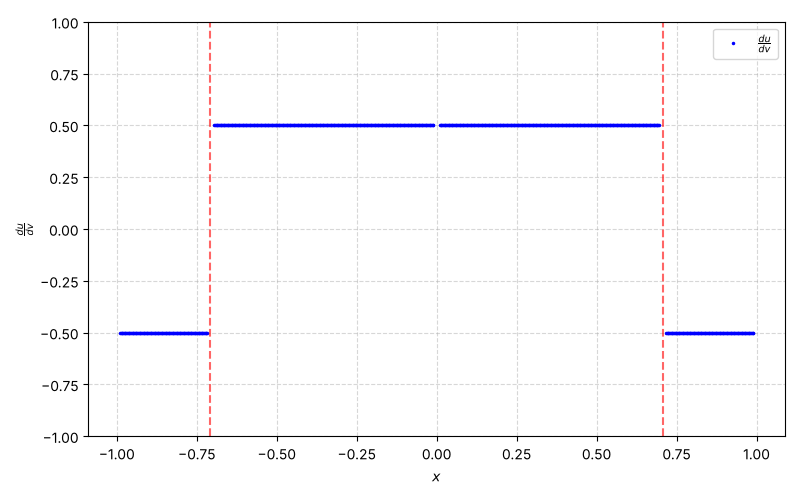
\includegraphics[width=0.75\linewidth]{figs/Derivative_Ratio.png}
    \caption{Plot of $\frac{du}{dv}$}
    \label{fig:EE26BTECHXXXXX-ratio}
\end{figure}

\item
If $y = x^x$, prove that $\dfrac{d^2y}{dx^2} - \dfrac{1}{y}\brak{\dfrac{dy}{dx}}^2 - \dfrac{y}{x} = 0$.
\par
\medskip
\solution
For $x > 0$, $y > 0$ and $\ln y = x\ln x$. From \eqref{eq:EE26BTECHXXXXX-logder},
\begin{align}
\frac{y^{\prime}}{y} = \brak{x\ln x}^{\prime} = 1 + \ln x
\\
\frac{y^{\prime\prime}}{y} - \brak{\frac{y^{\prime}}{y}}^2 = \brak{1 + \ln x}^{\prime} = \frac{1}{x}
\end{align}
Multiplying by $y$,
\begin{align}
y^{\prime\prime} - \frac{\brak{y^{\prime}}^2}{y} - \frac{y}{x} = 0
\end{align}
The following code verifies the solution.
\begin{lstlisting}[frame=single, basicstyle=\rmfamily, escapeinside={(*@}{@*)}]
(*@\makebox[\dimexpr\linewidth-2\fboxsep-2\fboxrule\relax][c]{codes/Log\_Derivative.py}@*)
\end{lstlisting}

\item
Find the intervals in which the function $f\brak{x} = 3x^4 - 4x^3 - 12x^2 + 5$ is
\begin{enumerate}
\item strictly increasing
\item strictly decreasing
\end{enumerate}
\par
\medskip
\solution
Differentiating,
\begin{align}
f^{\prime}\brak{x} = 12x^3 - 12x^2 - 24x = 12x\brak{x-2}\brak{x+1}
\end{align}
The critical points are $x = -1, 0, 2$. The sign of $f^{\prime}$ on each interval is given in \tabref{tab:EE26BTECHXXXXX-sign}.
\begin{table}[H]
\centering
\begin{tabular}{|c|c|c|}
\hline
Interval & Sign of $f^{\prime}\brak{x}$ & Nature of $f$ \\
\hline
$\brak{-\infty,-1}$ & $-$ & decreasing \\
\hline
$\brak{-1,0}$ & $+$ & increasing \\
\hline
$\brak{0,2}$ & $-$ & decreasing \\
\hline
$\brak{2,\infty}$ & $+$ & increasing \\
\hline
\end{tabular}
\caption{Sign of $f^{\prime}$}
\end{table}
From \eqref{eq:EE26BTECHXXXXX-monotone}, $f$ is
\begin{enumerate}
\item strictly increasing on $\brak{-1,0} \cup \brak{2,\infty}$
\item strictly decreasing on $\brak{-\infty,-1} \cup \brak{0,2}$
\end{enumerate}
The following code verifies the solution and generates \figref{fig:EE26BTECHXXXXX-incr}.
\begin{lstlisting}[frame=single, basicstyle=\rmfamily, escapeinside={(*@}{@*)}]
(*@\makebox[\dimexpr\linewidth-2\fboxsep-2\fboxrule\relax][c]{codes/Increasing\_Function.py}@*)
\end{lstlisting}
\begin{figure}[H]
    \centering
    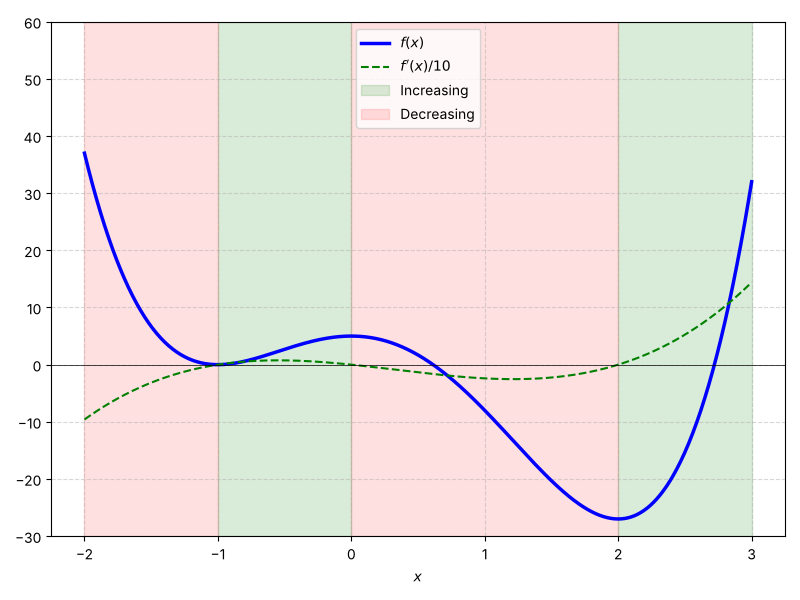
\includegraphics[width=0.75\linewidth]{figs/Increasing_Function.png}
    \caption{Intervals of increase and decrease}
    \label{fig:EE26BTECHXXXXX-incr}
\end{figure}

\item
Evaluate : $\displaystyle\int \dfrac{\sin^6 x + \cos^6 x}{\sin^2 x \cdot \cos^2 x}\, dx$
\par
\medskip
\solution
Let $a = \sin^2x$, $b = \cos^2x$, so that $a + b = 1$. From \eqref{eq:EE26BTECHXXXXX-cube-sum},
\begin{align}
\sin^6x + \cos^6x = a^3 + b^3 = 1 - 3ab
\end{align}
Then the integrand is
\begin{align}
\frac{1 - 3ab}{ab} = \frac{a+b}{ab} - 3 = \sec^2x + \cosec^2x - 3
\end{align}
From the standard integrals,
\begin{align}
\int \frac{\sin^6 x + \cos^6 x}{\sin^2 x \cos^2 x}\, dx = \tan x - \cot x - 3x + C
\end{align}
The following code verifies the solution.
\begin{lstlisting}[frame=single, basicstyle=\rmfamily, escapeinside={(*@}{@*)}]
(*@\makebox[\dimexpr\linewidth-2\fboxsep-2\fboxrule\relax][c]{codes/Trig\_Integral.py}@*)
\end{lstlisting}

\item
Find the particular solution of the differential equation $e^x\sqrt{1-y^2}\, dx + \dfrac{y}{x}\, dy = 0$, given that $y = 1$ when $x = 0$.
\par
\medskip
\solution
Multiplying by $\frac{x}{\sqrt{1-y^2}}$, the variables get separated:
\begin{align}
xe^x\, dx + \frac{y}{\sqrt{1-y^2}}\, dy = 0
\end{align}
Using \eqref{eq:EE26BTECHXXXXX-parts} with $u = x$, $dv = e^x\, dx$,
\begin{align}
\int xe^x\, dx = xe^x - \int e^x\, dx = \brak{x-1}e^x
\end{align}
Also, $\int \frac{y}{\sqrt{1-y^2}}\, dy = -\sqrt{1-y^2}$. Hence
\begin{align}
\brak{x-1}e^x - \sqrt{1-y^2} = C
\end{align}
Substituting $x = 0, y = 1$, $C = -1$. The particular solution is
\begin{align}
\sqrt{1-y^2} = \brak{x-1}e^x + 1
\end{align}
With $z = \sqrt{1-y^2}$, $z\, dz = -y\, dy$, and the equation reduces to $\frac{dz}{dx} = xe^x$, $z\brak{0} = 0$. The following code integrates this numerically and compares with the solution.
\begin{lstlisting}[frame=single, basicstyle=\rmfamily, escapeinside={(*@}{@*)}]
(*@\makebox[\dimexpr\linewidth-2\fboxsep-2\fboxrule\relax][c]{codes/Separable\_ODE.py}@*)
\end{lstlisting}

\item
Solve the following differential equation
\begin{align}
\brak{x^2 - 1}\frac{dy}{dx} + 2xy = \frac{2}{x^2 - 1}
\end{align}
\par
\medskip
\solution
Dividing by $x^2 - 1$,
\begin{align}
\frac{dy}{dx} + \frac{2x}{x^2-1}y = \frac{2}{\brak{x^2-1}^2}
\end{align}
Here $P = \frac{2x}{x^2-1}$, so $\mu = e^{\int P\, dx} = x^2 - 1$ (a constant sign factor cancels). From \eqref{eq:EE26BTECHXXXXX-ode-lin},
\begin{align}
\brak{x^2-1}y = \int \frac{2}{x^2-1}\, dx = \int \brak{\frac{1}{x-1} - \frac{1}{x+1}}\, dx
\end{align}
yielding
\begin{align}
y = \frac{1}{x^2-1}\sbrak{\ln\abs{\frac{x-1}{x+1}} + C}
\end{align}
The following code verifies the solution.
\begin{lstlisting}[frame=single, basicstyle=\rmfamily, escapeinside={(*@}{@*)}]
(*@\makebox[\dimexpr\linewidth-2\fboxsep-2\fboxrule\relax][c]{codes/Linear\_ODE.py}@*)
\end{lstlisting}

\item
Prove that, for any three vectors $\vec{a}, \vec{b}, \vec{c}$,
\begin{align}
\sbrak{\vec{a}+\vec{b}, \vec{b}+\vec{c}, \vec{c}+\vec{a}} = 2\sbrak{\vec{a}, \vec{b}, \vec{c}}
\end{align}
\par
\medskip
\solution
Let $\vec{M} = \myvec{\vec{a} & \vec{b} & \vec{c}}$. Then
\begin{align}
\myvec{\vec{a}+\vec{b} & \vec{b}+\vec{c} & \vec{c}+\vec{a}} = \vec{M}\vec{T}, \quad
\vec{T} = \myvec{1 & 0 & 1 \\ 1 & 1 & 0 \\ 0 & 1 & 1}
\end{align}
where the columns of $\vec{T}$ give the coefficients of $\vec{a}, \vec{b}, \vec{c}$. Now,
\begin{align}
\mydet{\vec{T}} = 1\brak{1 - 0} - 0 + 1\brak{1 - 0} = 2
\end{align}
From \eqref{eq:EE26BTECHXXXXX-triple} and \eqref{eq:EE26BTECHXXXXX-det-product},
\begin{align}
\sbrak{\vec{a}+\vec{b}, \vec{b}+\vec{c}, \vec{c}+\vec{a}} = \mydet{\vec{M}\vec{T}} = \mydet{\vec{M}}\mydet{\vec{T}} = 2\sbrak{\vec{a}, \vec{b}, \vec{c}}
\end{align}
The following code verifies the solution.
\begin{lstlisting}[frame=single, basicstyle=\rmfamily, escapeinside={(*@}{@*)}]
(*@\makebox[\dimexpr\linewidth-2\fboxsep-2\fboxrule\relax][c]{codes/Triple\_Product.py}@*)
\end{lstlisting}

\item
Show that the lines $\dfrac{x+1}{3} = \dfrac{y+3}{5} = \dfrac{z+5}{7}$ and $\dfrac{x-2}{1} = \dfrac{y-4}{3} = \dfrac{z-6}{5}$ intersect. Also find their point of intersection.
\par
\medskip
\solution
The lines are $\vec{x} = \vec{A}_1 + \lambda\vec{m}_1$ and $\vec{x} = \vec{A}_2 + \mu\vec{m}_2$ with
\begin{align}
\vec{A}_1 = \myvec{-1 \\ -3 \\ -5}, \vec{m}_1 = \myvec{3 \\ 5 \\ 7}, \vec{A}_2 = \myvec{2 \\ 4 \\ 6}, \vec{m}_2 = \myvec{1 \\ 3 \\ 5}
\end{align}
From \eqref{eq:EE26BTECHXXXXX-line-isect}, the augmented matrix is
\begin{align}
\augvec{2}{1}{3 & -1 & 3 \\ 5 & -3 & 7 \\ 7 & -5 & 11}
\xrightarrow[R_3 \to 3R_3 - 7R_1]{R_2 \to 3R_2 - 5R_1}
\augvec{2}{1}{3 & -1 & 3 \\ 0 & -4 & 6 \\ 0 & -8 & 12}
\xrightarrow{R_3 \to R_3 - 2R_2}
\augvec{2}{1}{3 & -1 & 3 \\ 0 & -4 & 6 \\ 0 & 0 & 0}
\end{align}
The ranks of the coefficient matrix and the augmented matrix are both $2$, so \eqref{eq:EE26BTECHXXXXX-consistent} holds and the lines intersect. Back-substitution gives
\begin{align}
\mu = -\frac{3}{2}, \quad 3\lambda = 3 + \mu \implies \lambda = \frac{1}{2}
\end{align}
The point of intersection is
\begin{align}
\vec{A}_1 + \lambda\vec{m}_1 = \myvec{\frac{1}{2} \\ -\frac{1}{2} \\ -\frac{3}{2}}
\end{align}
The following code verifies the solution and generates \figref{fig:EE26BTECHXXXXX-skew}.
\begin{lstlisting}[frame=single, basicstyle=\rmfamily, escapeinside={(*@}{@*)}]
(*@\makebox[\dimexpr\linewidth-2\fboxsep-2\fboxrule\relax][c]{codes/Skew\_Lines.py}@*)
\end{lstlisting}
\begin{figure}[H]
    \centering
    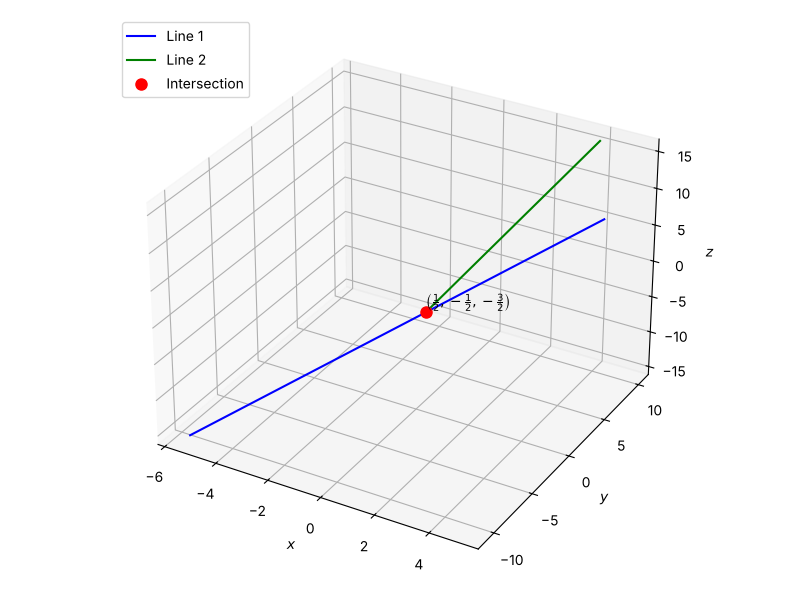
\includegraphics[width=0.75\linewidth]{figs/Skew_Lines.png}
    \caption{Intersecting lines}
    \label{fig:EE26BTECHXXXXX-skew}
\end{figure}

\item
Assume that each born child is equally likely to be a boy or a girl. If a family has two children, what is the conditional probability that both are girls? Given that
\begin{enumerate}
\item the youngest is a girl.
\item atleast one is a girl.
\end{enumerate}
\par
\medskip
\solution
Writing the outcomes as (elder, younger), the sample space is $\cbrak{GG, GB, BG, BB}$ with probability $\frac{1}{4}$ each. Let
\begin{itemize}
\item $A$: both are girls $= \cbrak{GG}$
\item $B$: the youngest is a girl $= \cbrak{GG, BG}$
\item $C$: at least one is a girl $= \cbrak{GG, GB, BG}$
\end{itemize}
Since $AB = AC = A$, from \eqref{eq:EE26BTECHXXXXX-cond},
\begin{align}
\pr{\cond{A}{B}} = \frac{\pr{A}}{\pr{B}} = \frac{1/4}{2/4} = \frac{1}{2}
\\
\pr{\cond{A}{C}} = \frac{\pr{A}}{\pr{C}} = \frac{1/4}{3/4} = \frac{1}{3}
\end{align}
The following code simulates the result.
\begin{lstlisting}[frame=single, basicstyle=\rmfamily, escapeinside={(*@}{@*)}]
(*@\makebox[\dimexpr\linewidth-2\fboxsep-2\fboxrule\relax][c]{codes/Conditional\_Probability.py}@*)
\end{lstlisting}

\item
Two schools P and Q want to award their selected students on the values of Discipline, Politeness and Punctuality. The school P wants to award \rupee{} $x$ each, \rupee{} $y$ each and \rupee{} $z$ each for the three respective values to its 3, 2 and 1 students with a total award money of \rupee{} 1,000. School Q wants to spend \rupee{} 1,500 to award its 4, 1 and 3 students on the respective values (by giving the same award money for the three values as before). If the total amount of awards for one prize on each value is \rupee{} 600, using matrices, find the award money for each value. Apart from the above three values, suggest one more value for awards.
\par
\medskip
\solution
The given conditions are
\begin{align}
3x + 2y + z = 1000, \quad 4x + y + 3z = 1500, \quad x + y + z = 600
\end{align}
or
\begin{align}
\myvec{3 & 2 & 1 \\ 4 & 1 & 3 \\ 1 & 1 & 1}\myvec{x \\ y \\ z} = \myvec{1000 \\ 1500 \\ 600}
\end{align}
Let the coefficient matrix be $\vec{A}$. Then
\begin{align}
\mydet{\vec{A}} = 3\brak{1-3} - 2\brak{4-3} + 1\brak{4-1} = -5 \neq 0
\end{align}
The adjoint of $\vec{A}$ gives
\begin{align}
\vec{A}^{-1} = \frac{1}{5}\myvec{2 & 1 & -5 \\ 1 & -2 & 5 \\ -3 & 1 & 5}
\end{align}
From \eqref{eq:EE26BTECHXXXXX-linsolve},
\begin{align}
\myvec{x \\ y \\ z} = \frac{1}{5}\myvec{2 & 1 & -5 \\ 1 & -2 & 5 \\ -3 & 1 & 5}\myvec{1000 \\ 1500 \\ 600}
= \myvec{100 \\ 200 \\ 300}
\end{align}
The awards are \rupee{} 100 for Discipline, \rupee{} 200 for Politeness and \rupee{} 300 for Punctuality. One more value that can be awarded is Honesty.
The following code verifies the solution.
\begin{lstlisting}[frame=single, basicstyle=\rmfamily, escapeinside={(*@}{@*)}]
(*@\makebox[\dimexpr\linewidth-2\fboxsep-2\fboxrule\relax][c]{codes/Matrix\_System.py}@*)
\end{lstlisting}

\item
Show that the semi-vertical angle of the cone of the maximum volume and of given slant height is $\cos^{-1}\dfrac{1}{\sqrt{3}}$.
\par
\medskip
\solution
For a fixed slant height $l$, from \eqref{eq:EE26BTECHXXXXX-cone}, the volume is a function of the height $h$:
\begin{align}
V\brak{h} = \frac{\pi}{3}\brak{l^2 h - h^3}
\end{align}
Differentiating,
\begin{align}
V^{\prime}\brak{h} = \frac{\pi}{3}\brak{l^2 - 3h^2} = 0 \implies h = \frac{l}{\sqrt{3}}
\\
V^{\prime\prime}\brak{h} = -2\pi h < 0
\end{align}
So $V$ is maximum at $h = \frac{l}{\sqrt{3}}$, from \eqref{eq:EE26BTECHXXXXX-monotone}. Using $h = l\cos\alpha$,
\begin{align}
\cos\alpha = \frac{h}{l} = \frac{1}{\sqrt{3}} \implies \alpha = \cos^{-1}\frac{1}{\sqrt{3}}
\end{align}
The maximum volume is $\frac{2\pi l^3}{9\sqrt{3}}$. The following code plots $V$ as a function of $\alpha$ in \figref{fig:EE26BTECHXXXXX-cone}.
\begin{lstlisting}[frame=single, basicstyle=\rmfamily, escapeinside={(*@}{@*)}]
(*@\makebox[\dimexpr\linewidth-2\fboxsep-2\fboxrule\relax][c]{codes/Cone\_Volume.py}@*)
\end{lstlisting}
\begin{figure}[H]
    \centering
    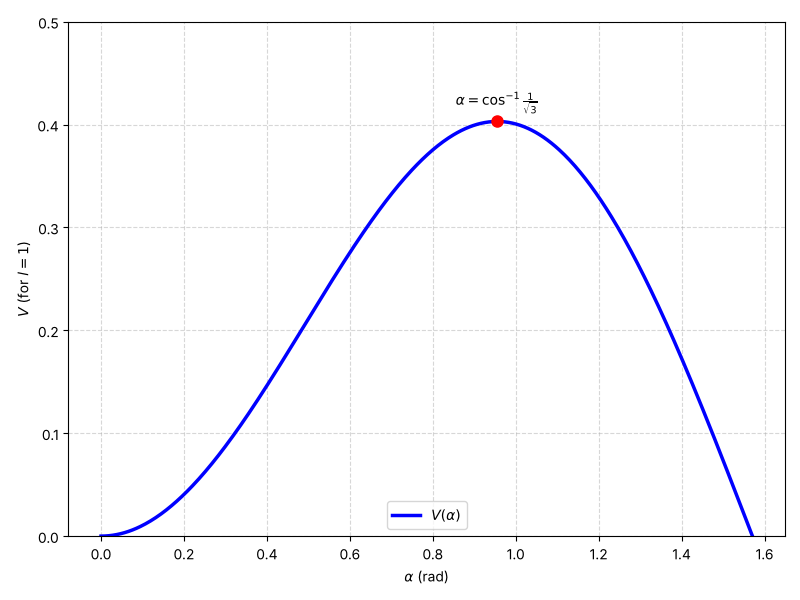
\includegraphics[width=0.75\linewidth]{figs/Cone_Volume.png}
    \caption{Volume of the cone versus $\alpha$}
    \label{fig:EE26BTECHXXXXX-cone}
\end{figure}

\item
Evaluate : $\displaystyle\int_{\pi/6}^{\pi/3} \dfrac{dx}{1 + \sqrt{\cot x}}$
\par
\medskip
\solution
Multiplying the numerator and denominator by $\sqrt{\sin x}$,
\begin{align}
I = \int_{\pi/6}^{\pi/3} \frac{\sqrt{\sin x}}{\sqrt{\sin x} + \sqrt{\cos x}}\, dx
\end{align}
Here $a + b = \frac{\pi}{6} + \frac{\pi}{3} = \frac{\pi}{2}$. From \eqref{eq:EE26BTECHXXXXX-king},
\begin{align}
I = \int_{\pi/6}^{\pi/3} \frac{\sqrt{\cos x}}{\sqrt{\cos x} + \sqrt{\sin x}}\, dx
\end{align}
Adding the two expressions of $I$,
\begin{align}
2I = \int_{\pi/6}^{\pi/3} dx = \frac{\pi}{3} - \frac{\pi}{6} = \frac{\pi}{6}
\implies I = \frac{\pi}{12}
\end{align}
The following code verifies the solution.
\begin{lstlisting}[frame=single, basicstyle=\rmfamily, escapeinside={(*@}{@*)}]
(*@\makebox[\dimexpr\linewidth-2\fboxsep-2\fboxrule\relax][c]{codes/Integral\_Symmetry.py}@*)
\end{lstlisting}

\item
Find the area of the region in the first quadrant enclosed by the $x$-axis, the line $y = x$ and the circle $x^2 + y^2 = 32$.
\par
\medskip
\solution
The line $y = x$ is $\theta = \frac{\pi}{4}$ and the circle is $r = \sqrt{32} = 4\sqrt{2}$. They meet at $\brak{4,4}$. The region is $0 \le r \le 4\sqrt{2}$, $0 \le \theta \le \frac{\pi}{4}$. From \eqref{eq:EE26BTECHXXXXX-polar-area},
\begin{align}
A = \int_{0}^{\pi/4}\int_{0}^{4\sqrt{2}} r\, dr\, d\theta
= \frac{\pi}{4}\cdot\frac{32}{2} = 4\pi
\end{align}
The following code computes the area and generates \figref{fig:EE26BTECHXXXXX-area}.
\begin{lstlisting}[frame=single, basicstyle=\rmfamily, escapeinside={(*@}{@*)}]
(*@\makebox[\dimexpr\linewidth-2\fboxsep-2\fboxrule\relax][c]{codes/Area\_Polar.py}@*)
\end{lstlisting}
\begin{figure}[H]
    \centering
    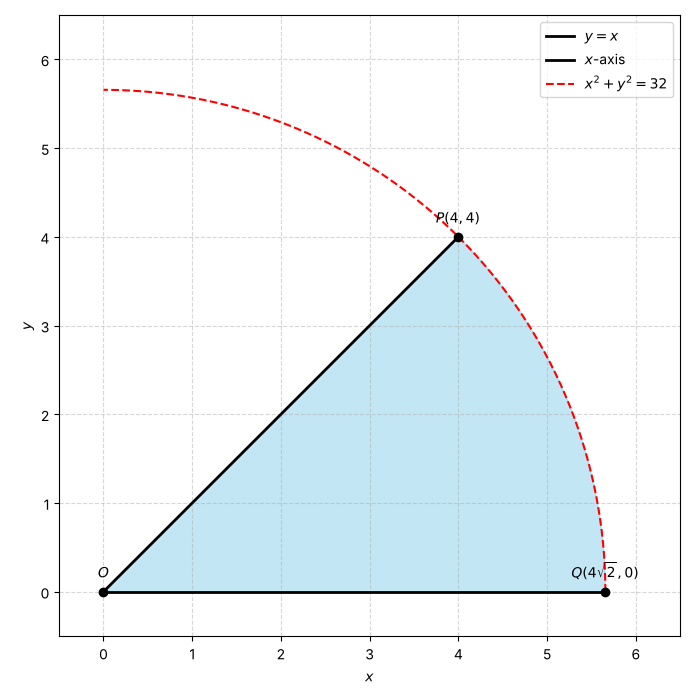
\includegraphics[width=0.60\linewidth]{figs/Area_Polar.png}
    \caption{Region enclosed by the $x$-axis, $y=x$ and the circle}
    \label{fig:EE26BTECHXXXXX-area}
\end{figure}

\item
Find the distance between the point $\brak{7, 2, 4}$ and the plane determined by the points $A\brak{2, 5, -3}$, $B\brak{-2, -3, 5}$ and $C\brak{5, 3, -3}$.
\par
\medskip
\solution
Let
\begin{align}
\vec{A} = \myvec{2 \\ 5 \\ -3}, \vec{B} = \myvec{-2 \\ -3 \\ 5}, \vec{C} = \myvec{5 \\ 3 \\ -3}, \vec{P} = \myvec{7 \\ 2 \\ 4}
\end{align}
Then $\vec{B} - \vec{A} = \myvec{-4 \\ -8 \\ 8}$ and $\vec{C} - \vec{A} = \myvec{3 \\ -2 \\ 0}$. From \eqref{eq:EE26BTECHXXXXX-plane-3pts},
\begin{align}
\myvec{-4 & -8 & 8 \\ 3 & -2 & 0}\vec{n} = \vec{0}
\xrightarrow[R_2 \to R_2 - 3R_1]{R_1 \to -\frac{R_1}{4}}
\myvec{1 & 2 & -2 \\ 0 & -8 & 6}
\xrightarrow[R_1 \to R_1 + \frac{R_2}{4}]{R_2 \to -\frac{R_2}{8}}
\myvec{1 & 0 & -\frac{1}{2} \\ 0 & 1 & -\frac{3}{4}}
\end{align}
so $n_1 = \frac{n_3}{2}$, $n_2 = \frac{3n_3}{4}$ and we can take
\begin{align}
\vec{n} = \myvec{2 \\ 3 \\ 4}, \quad c = \vec{n}^{\top}\vec{A} = 4 + 15 - 12 = 7
\end{align}
The plane is $\myvec{2 & 3 & 4}\vec{x} = 7$. From \eqref{eq:EE26BTECHXXXXX-plane-dist},
\begin{align}
d = \frac{\abs{14 + 6 + 16 - 7}}{\sqrt{4 + 9 + 16}} = \frac{29}{\sqrt{29}} = \sqrt{29}
\end{align}
The following code verifies the solution.
\begin{lstlisting}[frame=single, basicstyle=\rmfamily, escapeinside={(*@}{@*)}]
(*@\makebox[\dimexpr\linewidth-2\fboxsep-2\fboxrule\relax][c]{codes/Plane\_Distance.py}@*)
\end{lstlisting}

\item
A dealer in rural area wishes to purchase a number of sewing machines. He has only \rupee{} 5,760 to invest and has space for at most 20 items for storage. An electronic sewing machine cost him \rupee{} 360 and a manually operated sewing machine \rupee{} 240. He can sell an electronic sewing machine at a profit of \rupee{} 22 and a manually operated sewing machine at a profit of \rupee{} 18. Assuming that he can sell all the items that he can buy, how should he invest his money in order to maximize his profit? Make it as a LPP and solve it graphically.
\par
\medskip
\solution
Let $x$ electronic and $y$ manually operated machines be purchased, $\vec{x} = \myvec{x \\ y}$. The problem is
\begin{align}
\max Z = \myvec{22 & 18}\vec{x}
\quad \text{s.t.} \quad
\myvec{3 & 2 \\ 1 & 1}\vec{x} \le \myvec{48 \\ 20}, \quad \vec{x} \ge \vec{0}
\end{align}
where the first constraint is $360x + 240y \le 5760$. The feasible region in \figref{fig:EE26BTECHXXXXX-lpp} is a polygon. The vertex $B$ where the two constraints are tight is
\begin{align}
\myvec{3 & 2 \\ 1 & 1}\vec{x} = \myvec{48 \\ 20}
\implies \vec{x} = \myvec{1 & -2 \\ -1 & 3}\myvec{48 \\ 20} = \myvec{8 \\ 12}
\end{align}
The value of $Z$ at the vertices is given in \tabref{tab:EE26BTECHXXXXX-lpp}.
\begin{table}[H]
\centering
\begin{tabular}{|c|c|c|}
\hline
Vertex & $\brak{x,y}$ & $Z = 22x + 18y$ \\
\hline
$O$ & $\brak{0,0}$ & $0$ \\
\hline
$A$ & $\brak{16,0}$ & $352$ \\
\hline
$B$ & $\brak{8,12}$ & $392$ \\
\hline
$C$ & $\brak{0,20}$ & $360$ \\
\hline
\end{tabular}
\caption{Profit at the vertices}
\end{table}
From \eqref{eq:EE26BTECHXXXXX-corner}, the maximum profit is \rupee{} 392, when $8$ electronic and $12$ manually operated machines are purchased. The following code solves the LPP and generates \figref{fig:EE26BTECHXXXXX-lpp}.
\begin{lstlisting}[frame=single, basicstyle=\rmfamily, escapeinside={(*@}{@*)}]
(*@\makebox[\dimexpr\linewidth-2\fboxsep-2\fboxrule\relax][c]{codes/LPP.py}@*)
\end{lstlisting}
\begin{figure}[H]
    \centering
    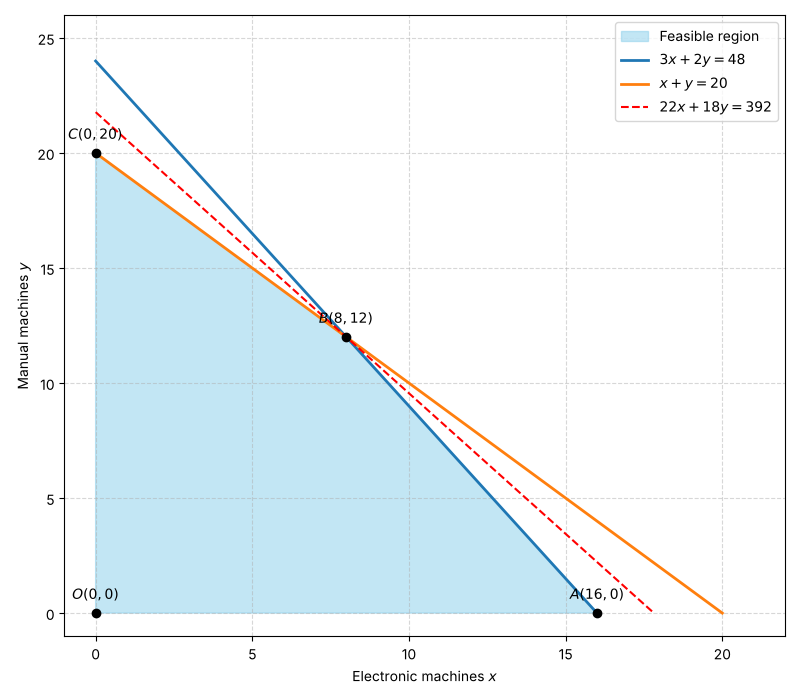
\includegraphics[width=0.75\linewidth]{figs/LPP.png}
    \caption{Feasible region and the optimal vertex}
    \label{fig:EE26BTECHXXXXX-lpp}
\end{figure}

\item
A card from a pack of 52 playing cards is lost. From the remaining cards of the pack three cards are drawn at random (without replacement) and are found to be all spades. Find the probability of the lost card being a spade.
\par
\medskip
\solution
Let
\begin{itemize}
\item $E_1$: the lost card is a spade, $\pr{E_1} = \frac{13}{52} = \frac{1}{4}$
\item $E_2$: the lost card is not a spade, $\pr{E_2} = \frac{3}{4}$
\item $A$: three spades are drawn from the remaining $51$ cards
\end{itemize}
If $E_1$ occurs, $12$ spades remain, and if $E_2$ occurs, $13$ spades remain. So
\begin{align}
\pr{\cond{A}{E_1}} = \frac{\comb{12}{3}}{\comb{51}{3}} = \frac{220}{\comb{51}{3}}, \quad
\pr{\cond{A}{E_2}} = \frac{\comb{13}{3}}{\comb{51}{3}} = \frac{286}{\comb{51}{3}}
\end{align}
From \eqref{eq:EE26BTECHXXXXX-bayes},
\begin{align}
\pr{\cond{E_1}{A}} = \frac{\frac{1}{4}\cdot 220}{\frac{1}{4}\cdot 220 + \frac{3}{4}\cdot 286}
= \frac{220}{1078} = \frac{10}{49}
\end{align}
The following code verifies the solution.
\begin{lstlisting}[frame=single, basicstyle=\rmfamily, escapeinside={(*@}{@*)}]
(*@\makebox[\dimexpr\linewidth-2\fboxsep-2\fboxrule\relax][c]{codes/Bayes.py}@*)
\end{lstlisting}
\end{enumerate}
